\section{Belgian mutual health insurance} \label{intro:health-insurance}
The Belgian health care insurance is a broad solidarity-based form of social insurance. Mutual health insurers are the legally-appointed bodies for managing and providing the Belgian compulsory health care and disability insurance. The Belgian sickness fund law of 1990 states that a main goal of mutualities is to promote the physical, psychological and social well-being of their members \citep{ziekenfondswet}.

Joining one of several mutual health insurers or, alternatively, the relief fund for sickness and disability insurance\footnote{In Dutch: Hulpkas voor Ziekte -en Invaliditeitsuitkering (HZIV).} is obliged for anyone who (i) starts working, (ii) is still studying at the age of 25 years or (iii) receives unemployment benefits. Among other things, mutual health insurers are responsible for refunding medical interventions, drug purchases and payments related to disability and pregnancy leave. To implement their operations, mutual health insurers dispose of large databases containing health expenditure records of all their respective members. 

This project was done in close collaboration with the National Alliance of Christian Mutualities (NACM).\footnote{In Dutch: Landsbond der Christelijke Mutualiteiten (LCM).} NACM  is the largest Belgian mutual health insurer with records of over 4.4 million persons and over 60\% and 40\% market share in Flanders and Belgium, respectively. All data extractions and analyses were done in-house at the department of medical management of NACM in its headquarters in Brussels under supervision of and upon request by the Chief Medical Officer.

We developed a screening system based exclusively on basic personal information (i.e., age, gender) and readily-available health expenditure records collected by NACM, without requiring any external input. Our approach is cheap, non-invasive and can be applied on a population-wide scale, making it a suitable initial screening procedure (cfr. Figure~\ref{intro:screening-funnel}). The relevant patient-centric information embedded in these records belongs to three key classes:
\begin{itemize}
\item \textbf{Basic biographical information} includes the member's age, gender, place of residence and, if deceased, the date of death. Limited information regarding social status is also available, e.g. whether a member is entitled to increased compensation or suffers from a chronic illness.
\item \textbf{Medical provisions} are encoded via a national nomenclature comprising over 20,000 unique codes. Each medical act yields one or several of these nomenclature codes. 
\item \textbf{Drug purchases} are registered automatically and are encoded per package or per unit when purchased in retail and hospital pharmacies, respectively. In both cases, the encoding contains information about both volume and active substances. 
\end{itemize}

Figure~\ref{intro:dataflow} depicts the main data exchanges in Belgian healthcare. Each healthcare provider manages its own subset of a patient's health data, which is usually not fully shared with other caregivers. In principle, the patient's \emph{global medical file} (GMF), which is managed by his or her general practitioner (GP), should be comprehensive. However, GMFs require caregivers to share data, which does not always occur, and puts a burden on GPs. In contrast, mutual health insurers dispose of all reimbursed claims data, regardless of the associated caregiver, which gives them an overview of all healthcare activities. Additionally, claims data are structured while communication between caregivers is often done through plain text. Data sharing is improving through initiatives like Vitalink\footnote{More information can be found at \url{http://www.vitalink.be/}.}, Hubs and Metahubs\footnote{\url{https://www.ehealth.fgov.be/nl/zorgverleners/online-diensten/hubs-metahub}}, though these are still in their infancy.

\begin{figure}[!h]
  \centering
  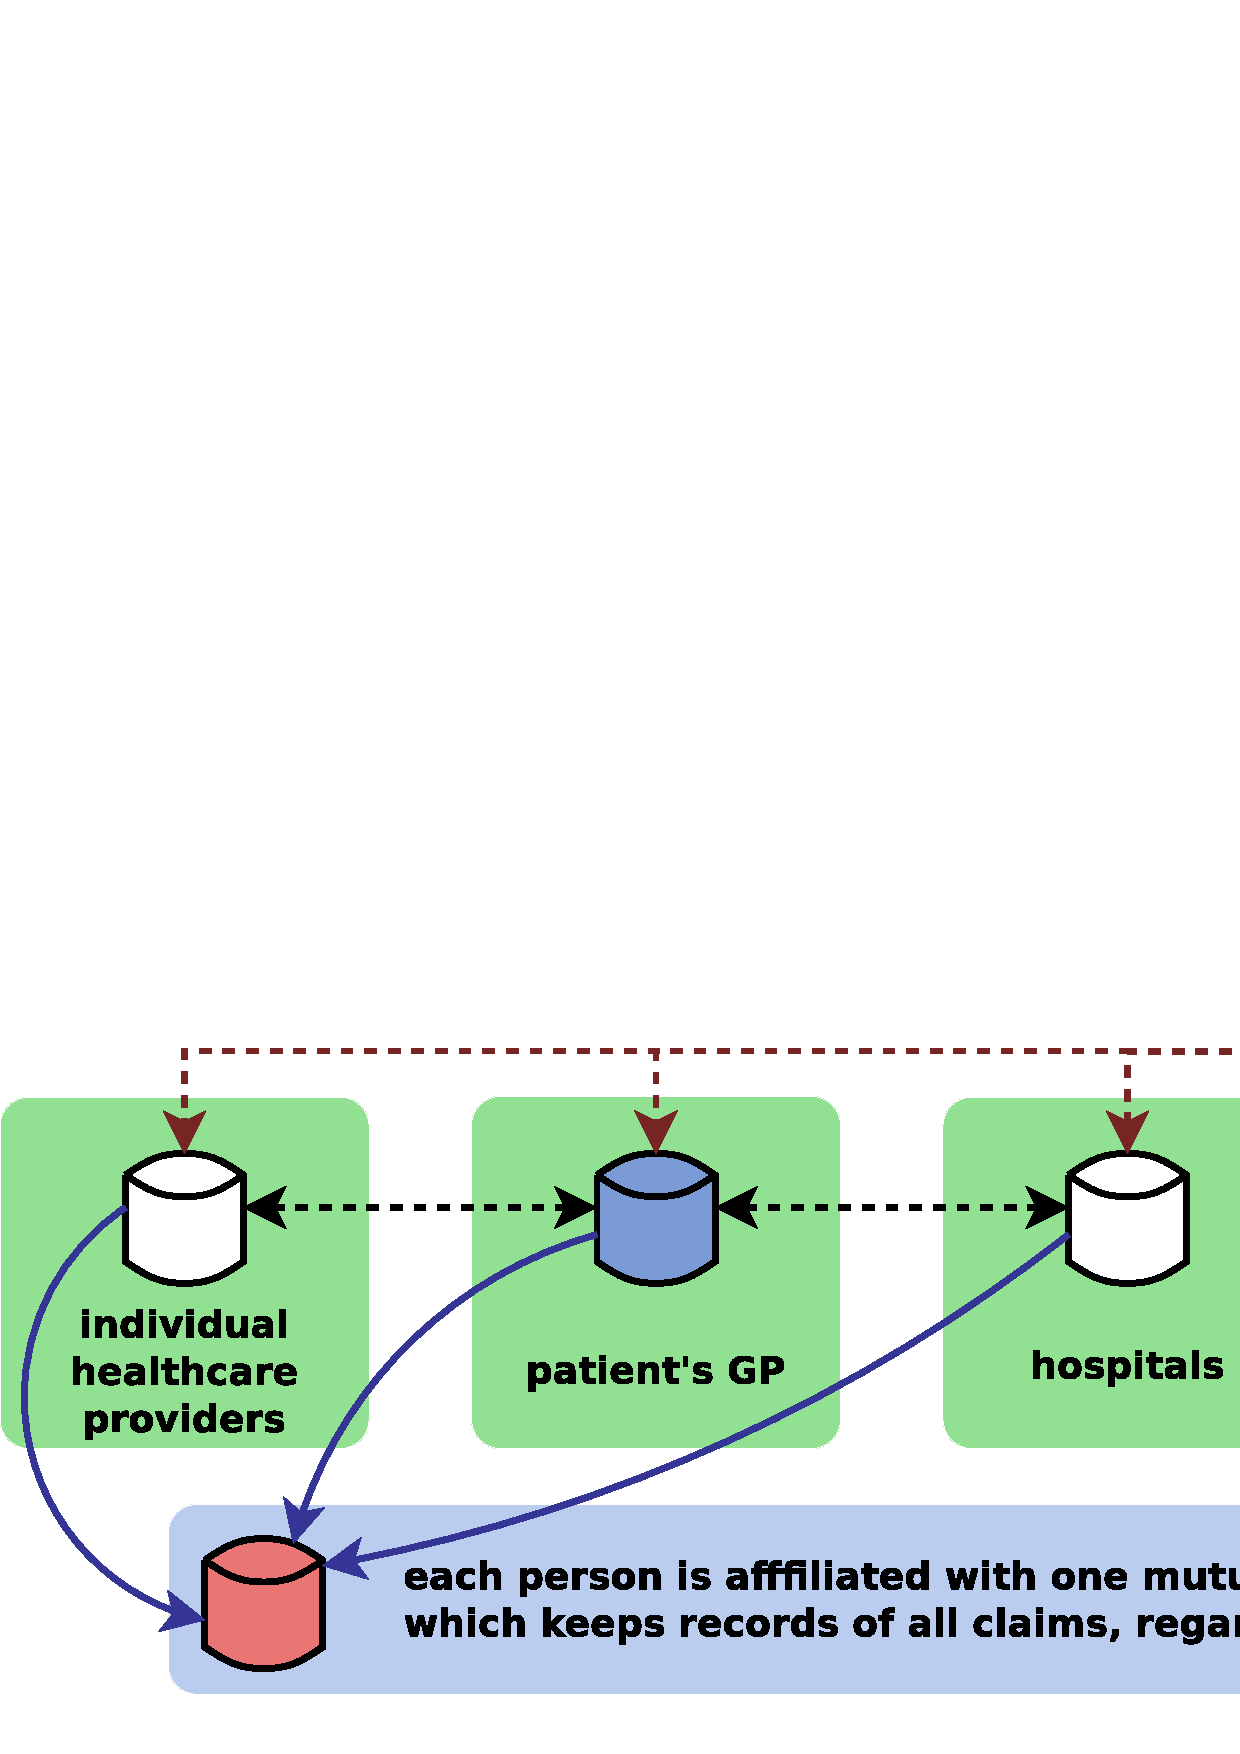
\includegraphics[width=0.95\textwidth]{dataflow.pdf}
 \caption{Data exchanges between caregivers in Belgian healthcare: mutual health insurers receive information from all stakeholders through claims, while other stakeholders often only have subsets of a patient's health data.}
  \label{intro:dataflow}
\end{figure}

The time-stamped records related to provisions and drug purchases enable constructing a medical resource-use timeline for each patient. As this constitutes the main source of information in our work we will discuss claims records related to provisions and drug purchases in more detail in Sections~\ref{intro:interventions}~and~\ref{intro:drugs}. Finally, we will briefly discuss the overall quality of health expenditure data.


\subsection{Data related to medical interventions} \label{intro:interventions}
Each distinct medical intervention is encoded in a national nomenclature that is maintained by the National Institute for Health and Disability Insurance (NIHDI)\footnote{In Dutch: Rijksinstituut voor ziekte -en invaliditeitsverzekering (RIZIV).} \citep{van2008financing}. After a consultation, patients receive a certificate indicating which provisions were performed (a green, white or blue slip). The patient can then file a claim to get (partially) refunded through his or her mutual health insurer. Refunds can be claimed up to two years after the date of the intervention, though most patients do this more swiftly. In some cases, a copayment system enables the caregiver to get paid directly by the health insurer, removing the need for the patient to claim refunds.

The list of nomenclature numbers can be consulted via the website of the NIHDI and currently comprises over 20,000 unique codes. The sheer number of codes indicates the fine granularity at which medical interventions are encoded, making it a valuable source of information. Codes can fall out of use when interventions get deprecated or because they get replaced by other codes that are often more specific in some sense.

However, the codes that identify interventions only carry limited information. Specifically, these codes are sufficiently detailed to know which intervention was performed, but do not contain any information regarding its outcome. For example, there are codes indicating blood tests, but the results of these tests are not available to the mutual health insurer. As such, nomenclature codes often serve as proxies for specific diseases, but essentially carry no direct information regarding diagnoses, indications or clinical parameters.

\subsection{Data related to drug purchases} \label{intro:drugs}
Drug purchases work via a copayment system in Belgium, in which the patient only pays his or her share at the time of purchase while the rest is already deducted automatically. As such, drug purchases are automatically recorded and known to health insurers without requiring the patient to explicitly claim refunds and are therefore implicitly complete.

Each drug package carries a \emph{Code Nationale Kode} (CNK) code which indicates the volume in the package and information about the drug itself including its active substances. Hence, these CNK codes carry enough information to map a drug purchase onto one or several codes of the internationally used Anatomical Therapeutic Chemical (ATC) classification system with an associated amount of Defined Daily Doses (DDDs). Tables to map CNK codes onto ATC codes are provided freely by the BCFI\footnote{In Dutch: Belgisch Centrum voor Farmacotherapeutische Informatie.} and the APB\footnote{In Dutch: Algemene Pharmaceutische Bond.}.

The ATC classification system is maintained by the World Health Organization and divides active substances into different groups based on the organ or system on which they act and their therapeutic, pharmacological and chemical properties \citep{world1996guidelines}. Each drug is classified in groups at 5 levels in the ATC hierarchy: fourteen main groups (1st level), pharmacological/therapeutic subgroups (2nd level), chemical subgroups (3rd and 4th level) and the chemical substance (5th level). Figure~\ref{intro:atc-example} illustrates the structure of ATC system for common antidiabetic drugs.

\begin{figure}[!h]
\dirtree{%
.1 \textsc{A}: alimentary tract and metabolism.
.2 \textsc{A10}: drugs used in diabetes.
.3 \textsc{A10A}: {\color{blue}insulins} and analogues.
.3 \textsc{A10B}: blood glucose-lowering drugs, excluding insulins.
.4 \textsc{A10BA}: {\color{blue}biguanides}.
.5 \textsc{A10BA02}: {\color{red}metformin}.
.4 \textsc{A10BB}: {\color{blue}sulfonylureas}.
.5 \textsc{A10BB01}: {\color{red}glibenclamide}.
.5 \textsc{A10BB08}: {\color{red}gliquidone}.
.5 \textsc{A10BB12}: {\color{red}glimepiride}.
.4 \textsc{A10BF}: {\color{blue}alpha-glucosidase inhibitors}.
.5 \textsc{A10BF01}: {\color{red}acarbose}.
.4 \textsc{A10BG}: {\color{blue}thiazolinediones}.
.5 \textsc{A10BG03}: {\color{red}pioglitazone}.
.4 \textsc{A10BH}: {\color{blue}dipeptidyl peptidase 4 (DPP-4) inhibitors}.
.5 \textsc{A10BH01}: {\color{red}sitagliptin}.
.5 \textsc{A10BH02}: {\color{red}vildagliptin}.
}
\caption{Example of the ATC hierarchy for common GLAs. A brief explanation of these different active substances is given in Appendix~\ref{intro:treatment}.} \label{intro:atc-example}
\end{figure}


\subsection{Quality of health expenditure data} \label{cmdata-quality}
Overall, health expenditure data can be considered complete, due to the clear financial incentive for patients and caregivers to file claims. The automated registration of drug purchases also contributes to this aspect.

A key benefit of health expenditure data is that it integrates resource-use from all medical sources (cfr. Figure~\ref{intro:dataflow}). Patients may consult multiple caregivers and institutions but each patient is affiliated to only one mutual health insurer at a time. Additionally, most Belgians never switch mutual health insurer. 

Health expenditure records give a fine-grained overview of patients' medical histories thanks to the detailed encoding of provisions and drug packages. However, the absence of data related to outcomes, diagnoses and clinical parameters constitutes an important limitation. In this regard, it must be noted that a lot of relevant information to screen for T2D is missing, such as glycated hemoglobin levels, lifestyle, BMI and potential genetic predisposition.

Health expenditure records prove extremely useful for retrospective observational studies, as is common in epidemiology. However, a certain lag exists between medical acts  and the appearance of associated records in health expenditure databases. For provision records, the maximum lag is two years, while for drug purchases the lag is less than half a year. These lags present problems for applications that require quasi real-time information, such as disease outbreak detection, but are less problematic for screening.

A disadvantage is that expenditure data may be noisy. Most sources of noise can be considered random and hence neglected, but some structural issues exist as well. Specific examples include abuse via overconsumption and fraud through \emph{upcoding}.\footnote{Upcoding refers to caregivers' wilfull reporting of wrong nomenclature codes, or codes corresponding to provisions that were never performed, in order to obtain higher refunds.} Such phenomena are known to plague healthcare systems in various countries and likely occur in Belgium as well to some extent \citep{silverman2004medicare,steinbusch2007risk,berta2010effects, Azguridiene12022015}.

Finally, it is worth noting that the potential of health expenditure data for clinical applications is also being investigated in other countries. A highly visible recent example was the Heritage Health Prize competition to identify patients who will be admitted to a hospital within the next year using historical claims data, with an impressive \$3,000,000 prize pool.\footnote{More information is available at \url{http://www.heritagehealthprize.com/}.}
